\section{Landmark Graph}
\begin{frame}{Phase A $\sim$ Definition and Recognition of Landmarks}
    \begin{itemize}
        \item Landmarks in this paper are \textbf{sensory landmarks};
            \begin{block}{Sensory landmarks}
                Location points where sensor readings present a distinct, stable, and identifiable change pattern
            \end{block}
        \item $\forall$ landmark $\exists$ 3 features:
            \begin{itemize}
                \item \textbf{Distinctiveness}: Unique change patterns distinguishable from surroundings;
                \item \textbf{Stability}: It doesn't change dynamically over time;
                \item \textbf{Identifiability}: Detectable by one or more sensors.
            \end{itemize}
        \item Mathematical definition: \( v = \langle (x, y), (R_1, \ldots, R_M) \rangle \)
            \begin{itemize}
                  \item $(x, y)$: coordinate of the landmark;
                  \item $(R_1, \dots ,R_M)$: detection rule in different types of sensor readings;
                  \item $M$ is the number of rules that this landmark possesses.
            \end{itemize}
    \end{itemize}
\end{frame}

\begin{frame}{Types of Landmarks: Accelerometer Landmark}
    \begin{columns}
        \begin{column}{.65\textwidth}
            \begin{itemize}
                \item Detects changes in motion state (e.g., walking to still);
                \item Example: Door locations where motion changes from walking to still and back to walking;
                \item Rule \( R_{acc} \):
                    \begin{itemize}
                        \item Pattern: Walking → Still → Walking;
                        \item Motion state \( m_t \) at time \( t \);
                        \item Window sizes \( K_1 \) and \( K_2 \).
                    \end{itemize}
            \end{itemize}
        \end{column}%
        \hfill%
        \begin{column}{.35\textwidth}
            \begin{figure}[!htb]
                \centering
                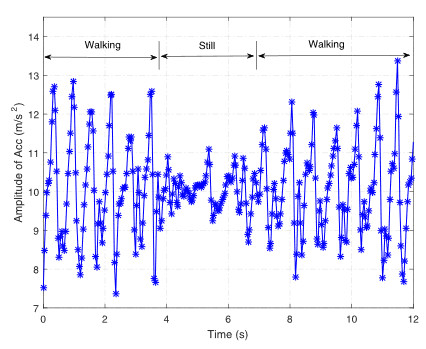
\includegraphics[width=\linewidth]{images/racc.jpg}
                \caption{Change in the amplitude of acceleration}
                \label{fig:racc}
            \end{figure}
        \end{column}
    \end{columns}
    \begin{alignteo}
        R_{acc} = (& loc_t | m_{t-K_1 : t} == walking\\
        & \&\& \, m_{t: t+K_2} == still\\
        & \&\& \, m_{t-K_2 : t + K_2 + K_1} == walking)
    \end{alignteo}
\end{frame}

\begin{frame}{Types of Landmarks: Gyroscope Landmark}
    \begin{columns}
        \begin{column}{.55\textwidth}
            \begin{itemize}
                \item Detects changes in walking direction (e.g., turns, corners) using magnetometer \& gyroscope;
                \item \redt{CON}: magnetometer readings are affected by ferromagnetic materials;
                \item Rule \( R_{gyro} \):
                    \begin{itemize}
                        \item \( \dot{\theta_t} \): gyroscope readings along the vertical direction;
                        \item Threshold \( \epsilon_{gyro} \) (\texttt{if} \( \dot{\theta_t} > \epsilon_{gyro}\) \texttt{then} location point is a potential gyroscope landmark).
                    \end{itemize}
            \end{itemize}
        \end{column}
        \begin{column}{.45\textwidth}
            \begin{figure}[t]
                \vspace{0pt}
                \centering
                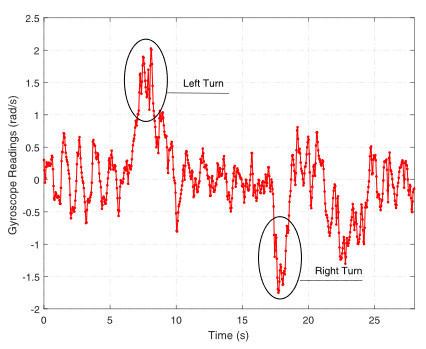
\includegraphics[width=\linewidth]{images/rgyro.jpg}
                \caption{Change in the gyroscope readings (z-axis)}
                \label{fig:rgyro}
            \end{figure}
            \begin{equation*}
                \tcbhighmath{
                    R_{gyro} = (loc_t |  \abs{\dot{\theta_t}} > \epsilon_{gyro})
                }
            \end{equation*}
        \end{column}
    \end{columns}
\end{frame}

\begin{frame}{Types of Landmarks: Barometer Landmark}
    \begin{itemize}
        \item Measures air pressure, which changes with altitude/height;\item Detects vertical movement (e.g., stairs, elevators);
        \item Example: Staircase or elevator entrances and exits.
    \end{itemize}
    \begin{figure}[t]
        \centering
        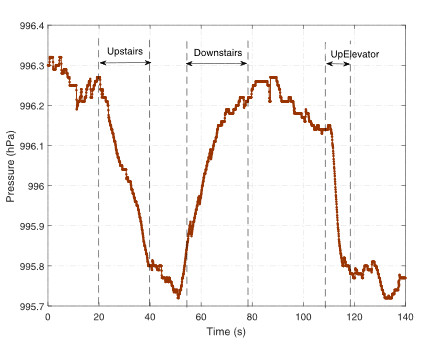
\includegraphics[width=0.5\linewidth]{images/rbaro.jpg}
        \caption{Change in the pressure when a user takes stairs or an elevator}
        \label{fig:rbaro}
    \end{figure}
\end{frame}

\begin{frame}{Types of Landmarks: Barometer Landmark}
    \begin{itemize}
        \item Rule \( R_{baro_1} \) for entrance:
            \begin{itemize}
                \item Horizontal → Vertical movement;
                \item \( p_i \): average value of the $i^{th}$ window of air pressure readings at the time $t$;
                \item thresholds \( \epsilon_{baro_1} \), \( \epsilon_{baro_2} \) to detect user's horizontal and vertical movement.
            \end{itemize}
    \end{itemize}

    \begin{alignteo}
        R_{baro_1} = (& loc_t| (\abs{p_i - p_{i-1}}) < \epsilon_{baro_1} \\
        & \&\& \abs{\sum_{j=i+1}^{i+K_{p_1}} (sgn(p_j - p_{j-1}))} == K_{p_1} \\
        & \&\& \abs{p_i+K_{p_1} - p_i} > \epsilon_{baro_2})
    \end{alignteo}
\end{frame}

\begin{frame}{Types of Landmarks: Barometer Landmark}
    \begin{itemize}
        \item Rule \( R_{baro2} \) for exit:
            \begin{itemize}
                \item Vertical → Horizontal movement.
            \end{itemize}
    \end{itemize}

    \begin{alignteo}
        R_{baro_2} = (& loc_t| (\abs{p_i - p_{i+1}}) < \epsilon_{baro_1} \\
        & \&\& \abs{\sum_{j=i-K_{p_2}}^{i} (sgn(p_j - p_{j-1}))} == K_{p_2} \\
        & \&\& \abs{p_i+K_{p_2} - p_i} > \epsilon_{baro_2})
    \end{alignteo}
\end{frame}

\begin{frame}{Types of Landmarks: WiFi Landmark}
    \begin{columns}
        \begin{column}{.55\textwidth}
            \begin{itemize}
                \item Detects location point that overhears the strongest RSS from an AP;
                \item Such point is typically stable, distinctive and identifiable;
                \item Rule \( R_{WiFi} \):
                    \begin{itemize}
                        \item Strongest RSS within a region;
                        \item RSS threshold \( \epsilon_{WiFi} \) (exclude local maxima).
                    \end{itemize}
            \end{itemize}
        \end{column}
        \begin{column}{.45\textwidth}
            \begin{figure}[t]
                \centering
                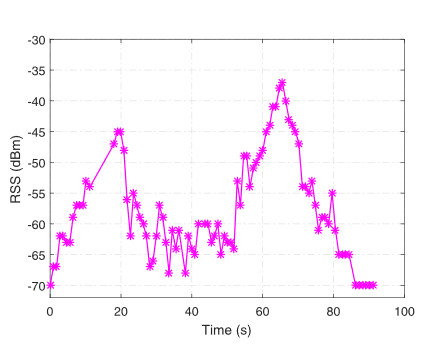
\includegraphics[width=\linewidth]{images/rwifi.jpg}
                \caption{RSS from an AP at different locations}
                \label{fig:rwifi}
            \end{figure}
        \end{column}            
    \end{columns}
        \begin{alignteo}
            R_{WiFi} = (& loc_t| (RSS_t == max(RSS_{t-{K_{WiFi}: t + K_{WiFi}}}))\\
            & \&\& RSS_t > \epsilon_{WiFi})
        \end{alignteo}
\end{frame}

\begin{frame}{Types of Landmarks: Light Landmark}
    \begin{columns}
        \begin{column}{.6\textwidth}
            \begin{itemize}
                \item Detects changes in light intensity using light sensor;
                \item Example: Projection location of a ceiling lamp;
                \item Rule \( R_{light} \):
                    \begin{itemize}
                        \item \( LX_t \): illuminance sensed by the sensor;
                        \item \( \epsilon_{light} \): threshold to exclude weak peaks of illuminance.
                    \end{itemize}
            \end{itemize}
        \end{column}
        \begin{column}{.4\textwidth}
            \begin{figure}[t]
                \centering
                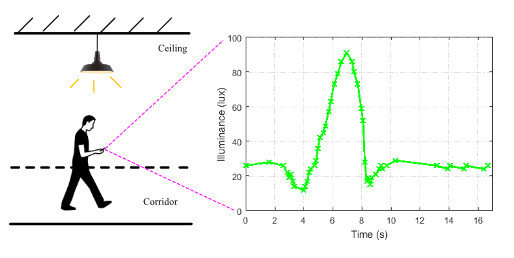
\includegraphics[width=\linewidth]{images/rlight.jpg}
                \caption{Change of luminance when a user passes a ceiling lamp}
                \label{fig:rlight}
            \end{figure}
        \end{column}            
    \end{columns}
    \begin{alignteo}
        R_{light} = (& loc_t| (LX_t == max(LX_{t-{K_{light}: t + K_{light}}}))\\
        & \&\& LX_t > \epsilon_{light})
    \end{alignteo}
\end{frame}

\begin{frame}{Phase B $\sim$ Construction of Initial Landmark Graph}
    \begin{itemize}
        \item \textbf{Landmark locations}:
            \begin{itemize}
                \item Doors, elevators, stairs, corners, turns (from floor maps);\item WiFi and light landmarks (learned from sensor readings and user trajectories).
            \end{itemize}
        \item \textbf{Constructing the corrisponding landmark graph}:\\
            \textbf{Ingredients}:
            \begin{itemize}
                \item Nodes: Landmarks;
                \item Edges: Accessible paths between landmarks;
                \item Graph Representation: $G = (V, E)$;
                \item $V$ = \{$v_1, \dots, v_N$\} (set of landmarks);
                \item $E$ = \{$e_1, \dots, e_M$\} (set of edges).
            \end{itemize}
        \item Each edge is represented by a tuple $e_i = \langle v_j, v_k, \theta_{jk}, d_i \rangle$ where:
            \begin{itemize}
                \item $v_j, v_k$: Set of landmarks;
                \item $\theta_{jk}$: Direction from $v_j$ to $v_k$;
                \item $d_i$: Distance between $v_j$ and $v_k$.
            \end{itemize}
    \end{itemize}
\end{frame}

\begin{frame}{Phase B $\sim$ Updating of Landmark Graph}
    \begin{itemize}
      \item \textbf{Initial Construction}:
        \begin{itemize}
            \item Based on floor plan;
            \item \textit{Incomplete}: lacks room-level details (e.g., furniture, desks);
            \item Cannot locate WiFi and light landmarks from floor plan.
        \end{itemize}
      \item \textbf{Learning New Landmarks}:
        \begin{itemize}
          \item Crowdsourcing: Collect $N$ user trajectories;
          \item Each trajectory contains $n_i$ potential landmarks \{$v_i^1, v_i^2, \dots, v_i^{n_i}$\};
          \item Total potential landmarks $N_0 = \sum_{i=1}^N n_i$.
        \end{itemize}
      \item \textbf{Potential Landmarks}:
        \begin{itemize}
          \item Location points satisfying detection rules;
          \item Not yet included in the current landmark graph.
        \end{itemize}
      \item \textbf{Updating Procedure}:
        \begin{itemize}
          \item \texttt{dist($c_i$, $c_j$)}: Euclidean distance between cluster centers;
          \item \texttt{rule}: Gets detection rule of a landmark;
          \item $d_c$: Distance threshold for merging clusters;
          \item $N_c$: Stability threshold for landmarks.
        \end{itemize}
    \end{itemize}
\end{frame}